\documentclass[12pt]{article}
\usepackage[english]{babel}
\usepackage{natbib}
\usepackage{url}
\usepackage[utf8x]{inputenc}
\usepackage{amsmath}
\usepackage{graphicx}
\graphicspath{{images/}}
\usepackage{parskip}
\usepackage{fancyhdr}
\usepackage{vmargin}
\setmarginsrb{3 cm}{2.5 cm}{3 cm}{2.5 cm}{1 cm}{1.5 cm}{1 cm}{1.5 cm}

\title{Emerging Technologies in Healthcare}								% Title
\author{21111038}								% Author
\date{25 Feb 2022}											% Date

\makeatletter
\let\thetitle\@title
\let\theauthor\@author
\let\thedate\@date
\makeatother

\pagestyle{fancy}
\fancyhf{}
\rhead{\theauthor}
\lhead{\thetitle}
\cfoot{\thepage}

\begin{document}

%%%%%%%%%%%%%%%%%%%%%%%%%%%%%%%%%%%%%%%%%%%%%%%%%%%%%%%%%%%%%%%%%%%%%%%%%%%%%%%%%%%%%%%%%

\begin{titlepage}
	\centering
    \vspace*{0.5 cm}
    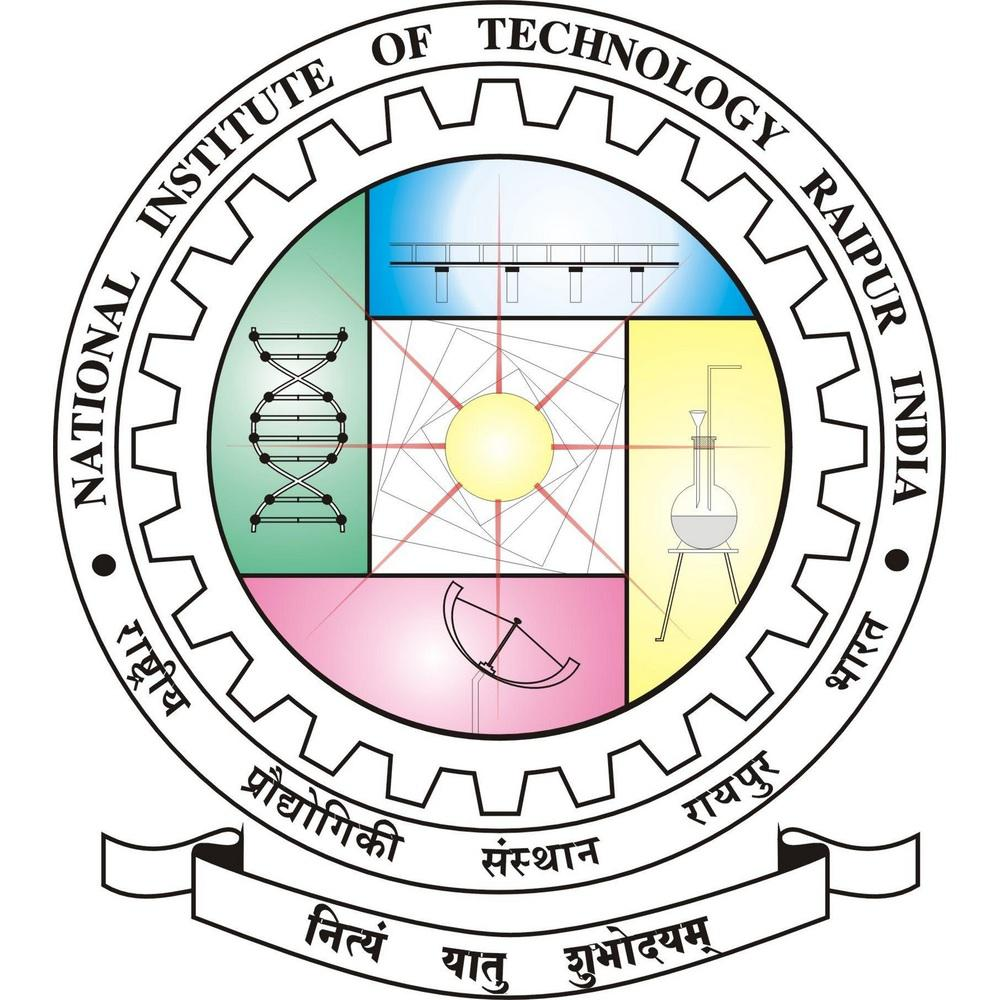
\includegraphics[scale = 0.17]{logo.jpg}\\[1.0 cm]	% University Logo
    \textsc{\LARGE  National Institute of Technology\newline\newline Raipur}\\[2.0 cm]	% University Name
	\textsc{\Large assignment 05}\\[0.5 cm]				% Course Code
	\rule{\linewidth}{0.2 mm} \\[0.4 cm]
	{ \huge \bfseries \thetitle}\\
	\rule{\linewidth}{0.2 mm} \\[1.5 cm]
	
	\begin{minipage}{0.4\textwidth}
		\begin{flushleft} \large
			\emph{Submitted To:}\\
			Saurabh Gupta\\
            Asst. Professor\\
            Department of Biomedical Engineering\\
			\end{flushleft}
			\end{minipage}~
			\begin{minipage}{0.4\textwidth}
            
			\begin{flushright} \large
			\emph{Submitted By :} \\
			Pradnya Manmode\\
            21111038\\
        First Semester\\
        Biomedical Engineering\\
		\end{flushright}
        
	\end{minipage}\\[2 cm]
	
	
    
    
    
    
	
\end{titlepage}


\title{ASSIGNMENT 05}
\maketitle

\indent
Digitalization has sped up transformation in industries. Today, equipment and processes are benefiting from new technologies, which are increasing productivity and efficiency across sectors. The global healthcare sector has also gained from these emerging trends. While the adoption rate is still slow, it is a boon to patients and doctors alike.

Healthcare technologies are diverse and encompass devices, medicines, vaccines, procedures, and systems to streamline operations, trim costs, and improve the quality of care delivered. Artificial intelligence (AI), blockchain, robotics, bio-printing, and nanotechnology are among the most promising technologies in the healthcare space.

New technology in healthcare includes supportive, educational, information, organizational, rehabilitative, therapeutic, preventive, and diagnostic solutions that improve patient access and healthcare provider capabilities. Virtual concierge, artificial intelligence, voice search, and virtual and augmented reality are promising emerging technologies for 2021.

\section{AI:}
Healthcare technologies are diverse and encompass devices, medicines, vaccines, procedures, and systems to streamline operations, trim costs, and improve the quality of care delivered. Artificial intelligence (AI), blockchain, robotics, bio-printing, and nanotechnology are among the most promising technologies in the healthcare space.
Atomwise uses AI to determine the best candidates for pre-clinical drug trials and analyzes billions of compounds to find the most effective drugs, thus reducing research time.
\section{Blockchain:}
This technology is expected to completely transform the collection and storage of medical history. Not only it would be easier to store information and access it through blockchain, but security threats would also be minimized. It would allow doctors to access the entire medical history of a patient, including any genetic illnesses and allergies, allowing them to customize treatment to provide the best possible care. The concept of blockchain for healthcare is still under development.
\section{Robotics:}
Robots were used medically for the first time in 1985. Since then, their role has expanded in this sector. Robots are mostly used in surgeries and to some extent in procedures such as laparoscopy, neurosurgery, orthopedic surgery, emergency response, and minimally invasive operations. The technology also has wearables such as robotic prostheses or exoskeletons that help with mobility issues in those suffering from missing or paralyzed limbs. Robots also gaining popularity as companions for the elderly or child patients.
\section{Nanotechnology:}
Nanotechnology for the healthcare space has been under development for a long time now. It studies molecular structure to develop precise devices and medicines. Some of developments using nanotechnology include nanorobots and nanomedicines. In 2018, an electronic pill was developed using nanotechnology; the pill can be controlled after release in the patient’s body to relay diagnostic details or to release drugs in a specific section of the body. Currently, the technology is used to make smart patches that can monitor wounds and stimulate rapid healing. Most of this application is still under research.
\section{3D bioprinting:}
 Another technological innovation for the healthcare space is 3D bioprinting. The global bioprinting market could have investments of almost USD 1.8 billion by 2027. With the help of DNA analysis, bio-printing can regenerate and replace several body parts, bones, and tissue. Recently, a research team developed a method to 3D-print living skin and blood vessels. This is a great breakthrough for skin grafts for burn victims. 3D-print prosthetics are also a boon for patients with missing limbs.
 
 \indent
 The examples mentioned here are just a few of those emerging in the global healthcare sector. While some have found acceptance, others are still at the development stage. There remains scope for more innovations and techniques, many of which are currently yet being studied. These technologies are reshaping the healthcare sector and its future. 
 \\
 The emergence of new technology has a significant impact on healthcare. The very objective of digitalization in this space is to improve the quality of healthcare provided while reducing stress on physicians.


\end{document}
